\title{CS251 Assignment 8}
\author{Sahil Dhull (160607)}
\documentclass{article}
\usepackage{graphicx}
\begin{document}
\maketitle

\clearpage
\begin{figure}
\includegraphics[width=\linewidth]{scatter1.eps}
\caption{1 Thread}
\label{fig:Scatter1 graph}
\end{figure}
\noindent
Scatter plot of time taken for execution v/s Number of
elements when the number of threads=1. \\
X-axis holds the number of elements and
Y-axis displays the time taken correspondingly.\\
There are some regions of high point density in the graphs.
\clearpage

\begin{figure}
\includegraphics[width=\linewidth]{scatter2.eps}
\caption{2 Threads}
\label{fig:Scatter2 graph}
\end{figure}
\noindent
Scatter plot of time taken for execution v/s Number of
elements when the number of threads=2. \\
X-axis holds the number of elements and
Y-axis displays the time taken correspondingly.\\
There are some regions of high point density in the graphs.
\clearpage

\begin{figure}
\includegraphics[width=\linewidth]{scatter3.eps}
\caption{4 Threads}
\label{fig:Scatter3 graph}
\end{figure}
\noindent
Scatter plot of time taken for execution v/s Number of
elements when the number of threads=4. \\
X-axis holds the number of elements and
Y-axis displays the time taken correspondingly.\\
There are some regions of high point density in the graphs.
\clearpage

\begin{figure}
\includegraphics[width=\linewidth]{scatter4.eps}
\caption{8 Threads}
\label{fig:Scatter4 graph}
\end{figure}
\noindent
Scatter plot of time taken for execution v/s Number of
elements when the number of threads=8. \\
X-axis holds the number of elements and
Y-axis displays the time taken correspondingly.\\
There are some regions of high point density in the graphs.
\clearpage

\begin{figure}
\includegraphics[width=\linewidth]{scatter5.eps}
\caption{16 Threads}
\label{fig:Scatter5 graph}
\end{figure}
\noindent
Scatter plot of time taken for execution v/s Number of
elements when the number of threads=16. \\
X-axis holds the number of elements and
Y-axis displays the time taken correspondingly.\\
There are some regions of high point density in the graphs.
\clearpage

\begin{figure}
\includegraphics[width=\linewidth]{lineplot.eps}
\caption{linegraph}
\label{fig:Line graph}
\end{figure}
\noindent
This is a line graph of average time taken for execution v/s Number of
elements. \\
X-axis holds the number of elements and
Y-axis displays the time taken correspondingly. \\
Different lines represent different no. of threads {1,2,4,8,16}.\\
Lines are of different color.
\clearpage

\begin{figure}
\includegraphics[width=\linewidth]{bar.eps}
\caption{Bargraph}
\label{fig:Average Speedup graph}
\end{figure}
\noindent
This is a bar graph of average time of execution where ratio is taken between average time for k threads vs average time for 1 thread, \\
X-axis holds the number of elements and number of threads {1,2,4,8,16} and Y-axis displays the ratio w.r.t 1
thread.\\

\clearpage

\begin{figure}
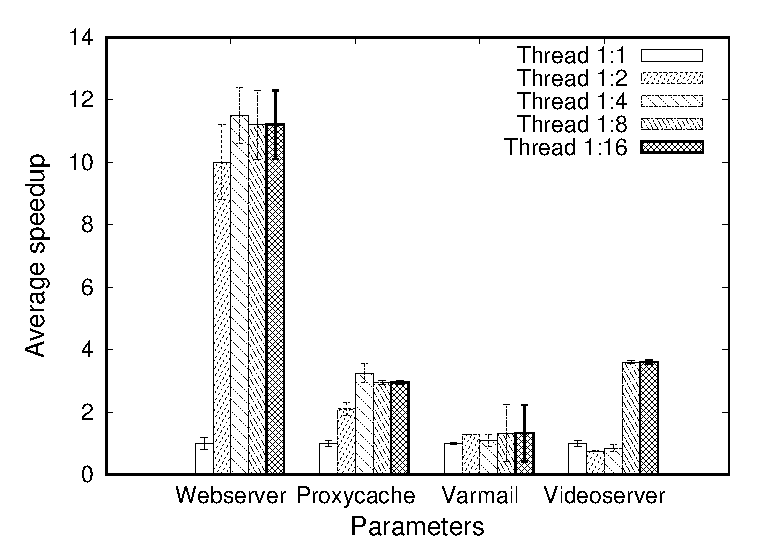
\includegraphics[width=\linewidth]{err.eps}
\caption{bargraph variance}
\label{fig:Error graph}
\end{figure}
\noindent
This is an error bar graph of average time of execution where ratio is taken between average time for k threads vs average time for 1 thread, \\
X-axis holds the number of elements and number of threads {1,2,4,8,16} and Y-axis displays the ratio(speed)
w.r.t 1 thread and also its variance.

\end{document}
